\documentclass[12pt, svgnames]{article}

\usepackage{fullpage}
\usepackage[round,numbers]{natbib}
\usepackage{multirow}
\usepackage{booktabs}
\usepackage{graphicx}
\usepackage{float}
\usepackage{../ltx/edcomms}
\usepackage{../ltx/setupComments}
\usepackage{hyperref}
\usepackage{geometry}
\usepackage{changepage}
\usepackage{adjustbox}
\usepackage{graphicx}
\usepackage[section]{placeins} % Prevents floats from floating across sections
\usepackage{tabularx}
\usepackage{amsfonts}
\usepackage{glossaries}
\usepackage{multirow} %% Used for Traceability matrix
\usepackage{listings}
\usepackage{calc}
\usepackage[simplified]{pgf-umlcd}
\usepackage[section]{placeins}
\usepackage{enumitem}

\usetikzlibrary{arrows.meta}
\usetikzlibrary{calc}
\usetikzlibrary{positioning}


\let\Oldsubsection\subsection
\renewcommand{\subsection}{\FloatBarrier\Oldsubsection}
\let\Oldsubsubsection\subsubsection
\renewcommand{\subsubsection}{\FloatBarrier\Oldsubsubsection}

%\usepackage{amssymb}
\newcounter{acnum}
\newcommand{\actheacnum}{AC\theacnum}
\newcommand{\acref}[1]{AC\ref{#1}}

\newcounter{ucnum}
\newcommand{\uctheucnum}{UC\theucnum}
\newcommand{\uref}[1]{UC\ref{#1}}

\newcounter{mnum}
\newcommand{\mthemnum}{M\themnum}
\newcommand{\mref}[1]{M\ref{#1}}
\makeglossary


% math things
\newcommand{\ra}{$\rightarrow$}



% 
\definecolor{grey}{RGB}{185,185,185}
\definecolor{applegreen}{rgb}{0.55, 0.71, 0.0}
\lstset{ %
  language=Haskell, morekeywords = {family, kind, pattern, expression},
  literate=
  {+}{{$+$}}1
  {/}{{$/$}}1 
  {*}{{$*$}}1 
  {=}{{$=\,\,\,$}}1
  {==}{{$==$}}1 
  %{/=}{{$\not\equiv$}}2
  {==}{{$\equiv$}}2
  {/=}{{$\not\equiv$}}2
  {>}{{$>$}}1 
  {<}{{$<$}}1 
  {\\}{{$\lambda$}}1
  {\\\\}{{\char`\\\char`\\}}1
  {>>}{$>>$}2 
  {:>>=}{{$:>>=$}}2
  %% {>>=}{{\hspace{6pt}\texttt{$>>=$}\hspace{6pt}}}2
  {->}{{$\rightarrow$} }2 
  {>=}{{$\geq$}}2 {<-}{{$\leftarrow$}}2
  {<=}{{$\leq$}}2 {=>}{{$\Rightarrow$} }2
  {|}{{$\mid$}}1 
  {forall}{{$\forall$}}1
  {exists}{{$\exists$}}1 
  {Nat}{{$\mathbb{N}$}}1
  {:\~:}{{$\equiv$}}2
  {\~}{{$\equiv$}}2
  {`In`}{{$\in$}}1
  {.}{{$\circ$\,\,}}1
  ,
  escapeinside={\%*}{*)},
  deletekeywords={>>,>>=,mapM,mapM_,putStrLn,putStr,toInt,show,and,sequence,String,Bool,True,False,Maybe,id,Show,Ordering},
  morekeywords={forall, ::, :},
  postbreak={},
  breaklines=true,                
  breakatwhitespace=true,
  %postbreak={  \mbox{\textcolor{grey}{$\rightarrow$}} },
  breakindent = 0pt,
  breakautoindent = true,
  %moredelim=[is][\itshape]{"}{"},
  morestring=[b]",
  mathescape
}

\newcommand{\hstype}[2][0pt]{\attribute{\hspace*{#1}\lstinline[mathescape]|#2|}}

\newcommand{\hstypectr}[1]{\attribute{\hspace*{10pt}\lstinline[mathescape]|#1|}}

\newcommand{\hsfunc}[2][0pt]{\operation{\hspace*{#1}\lstinline[mathescape]|#2|}}

%% \tikzset{>=latex}

\begin{document}

\title{\vspace*{3cm} Module Guide for ECA Rules for Ampersand} 
\author{Yuriy Toporovskyy (toporoy)\\ Yash Sapra (sapray) \\ Jaeden Guo (guoy34)}
%%Yuriy Toporovskyy (toporoy) \\ Yash Sapra (sapray) \\ Jaeden Guo (guoy34)}
\date{February 24th,\ 2016} 


\maketitle
\newpage
\vspace*{1cm}
\begin{table}[ht!]\begin{center}
        \caption{Revision History}  
        \begin{tabular}{|c|c|c|}\hline
            \textbf{Author} & \textbf{Date} & \textbf{Comments} \\\hline 
            Yash Sapra & 24 / 02 / 2016 & Initial draft\\\hline
	 Jaeden Guo & 27/ 02 / 2016 & Update and merge \\\hline
	 Yash Sapra & 28/ 02 / 2016 & Modifications to several sections \\\hline
	 Yuriy Toporovskyy & 28/ 02 / 2016 & Addition of UML diagrams \\\hline
	 Yuriy Toporovskyy & 29/ 02 / 2016 & Major changes (diagrams, explanations, organization) \\\hline
	 Yash Sapra & 29/ 02 / 2016 & Proof reading \\\hline
        \end{tabular}
    \end{center}\end{table}
\newpage

\tableofcontents

\newpage

\section{Introduction}\label{intro}
%TODO: edit for grammar, spelling, context, flow, watch for contractions
\subsection{Description}

This document details the module system of EFA, as well as the design principles
which guided said module system. EFA, as well as the core Ampersand system, is
currently in active development where changes occur frequently. Commonly
accepted practice for this situation is to decompose modules based on the
principle of abstraction, where unnecessary information in hidden for the
benefit of designers and maintainers\citep{modStruct,Parnas1972}.

Our design follows the principles laid out by \citep{modStruct}, which can be summarized as follows:
\begin{itemize}
\item Unnecessary design details are omitted for simplicity.
\item Each module is broken down based on hierarchy with no overlap of functionality.
\item All our modules are \emph{Open Modules}, that is, they are available for extension in the future.
\item Reference materials are provided for external libraries but details of
  their implementation are not included here. 
\end{itemize}

The language of implementation is Haskell. The primary reason for using Haskell
is that the existing Ampersand system is largely written in Haskell. However, we
leverage the full power of the Haskell type system in order to encode as many
invariants in Haskell as possible. In particular, we use many modern features of
the Glasgow Haskell Compiler (GHC) in order to do so. However, the particular
features, as well as how and where they are used, are considered an
implementation detail that is not relevant to the design of EFA.

\subsection{Scope}
The purpose of this document is to outline the implementation details of the 
EFA project described in the Problem Statement.
EFA is responsible for generating SQL Statements from ECA rules that will 
be used to fixed any violated invariants in the Ampersand prototype. 
The document will serve as a referral document for future software development in the Ampersand project.

\subsubsection{Intended Audience}
This document is designed for:
\paragraph{New project members:}
This document is designed to help introduce new Ampersand users to EFA 
(ECA rules for Ampersand). It provides a basic structure that allows 
individuals to quickly access the information they seek.
   
\paragraph{Maintainers \& Designers:} The structure of this module guide will 
help maintainers rationalize where changes should be made in order to 
accomplish their intended purpose. Furthermore, the design document will act as 
a guide to EFA for future designers of Ampersand.

\section{Anticipated and Unlikely Changes}
\subsection{Anticipated Changes}
It is likely that EFA will require changes to the front-end interface. This 
addition may include a protocol that will connect the front-end interface to 
back-end functions, which will give the user more control. In addition, ECA 
rules are not static and may change over time, if changes do take place those 
changes will need to be incorporated into EFA's future releases. 

Thus far anticipated changes include:

\begin{enumerate}[label=\textbf{AC\arabic*:}]
    \item New front-end interface.
    \item Addition or elimination of ECA rules.
    \item The algorithm used for EFA.
    \item The format of output.
    \item The format of input parameters.
    \item Integration of front-end interface to back-end modules.
    \item Testing for individual modules and internal systems.
\end{enumerate}

\subsection{Unlikely Changes} 

These unlikely changes include the things that will remain unchanged in the 
system, and also changes that would not affect EFA. 

\begin{enumerate}[label=\textbf{UC\arabic*:}]
    \item There will always be a source of input data external to the 
    software.
    \item Results will always be provably correct.
    \item The implementation language must be the same as that which is 
    used for building the Ampersand system.
    \item The format of initial input data and associated markers for 
    data association.
    \item Type of output data will always be a SQL query.
\end{enumerate}


%%%%%%%%%%%%%%%%%%%%%
%%% Section - System Architecture %%%%%
%%%%%%%%%%%%%%%%%%%%%
\newpage
\section{System Architecture} \label{SystemArch}

This section provides an overview of the module design. The module design is
detailed with UML-like class diagrams. However, UML class diagrams are typically
used to describe the module systems of object-oriented programs, as opposed to
functional programs. Many of the components of the traditional UML class
diagram are inapplicable to functional programs; therefore, we detail our
modifications to the UML class diagram syntax in section~\ref{subsec:ModuleSyntax}. 

Furthermore, the syntax used to describe types and data declarations is not
actual Haskell syntax. The syntax shares many similarities, but several changes
to the syntax are made in this document in order to present the module hierarchy
in a clear manner. These changes are also detailed, in section~\ref{subsec:HaskellSyntax}. 


\subsection{Haskell-like Syntax Description}\label{subsec:HaskellSyntax}

This section details the syntax used to describe the module system of
Ampersand. This syntax largely borrows from actual Haskell syntax, and from the
Agda programming language \cite{agda}. Agda is a dependantly typed functional
language, and since a large part of our work deals with ``faking'' dependant
types, the syntax of Agda is conducive to easy communication of our module system. The
principle of faking dependant types in Haskell is detailed in
Hasochism~\cite{hasochism} (a portmanteau of Haskell and masochism, because
purportedly wanting to fake dependant types in Haskell is masochism). While the
implementation has since been refined many times over, the general approach is still the
same, and will not be detailed here.

While the changes made to the Haskell syntax are reasonably complex, the ensuing 
module description becomes vastly simplified. This section is meant to be used
as a reference - in many cases, the meaning of a type is self-evident. 

\subsubsection*{Types and kinds}
In the way that a type classifies a set of values, a kind classifies a set of
types. Haskell permits one to define algebraic data types, which are then ``promoted''
to the kind level. This permits the type constructor of the datatype to be used
as a kind constructor, and for the value constructors to be used as type constructors. 
In every case in our system, when we define a datatype and use the promoted version,
we never use the \emph{unpromoted} version. That is, we define types which are never
used as types, only as kinds, and constructors which are never used as value constructors,
only type constructors. We write \,\,\,\lstinline!X : A -> B -> $\ldots$ -> Type!\,\,\, to denote
a regular data type, and \,\,\,\lstinline!Y : A -> B -> $\ldots$ -> Kind!\,\,\, to denote a datatype
which is used exclusively as a kind. 

\subsubsection*{Dependant types}
The syntax used to denote a ``fake'' dependant type in our model is the same 
as used to denote a real dependant type in Agda. \lstinline!(x : A) -> B! is the function
from $x$ to some value of type $B$, where $B$ can mention $x$. This nearly looks like a 
real Haskell type - in Haskell, the syntax would be \texttt{forall (x :: A) . B}. However, 
the semantics of these two types are vastly different - the former can pattern match
on the value of $x$, while the latter cannot. 

In certain cases, it may be elucidating to see the \emph{real} Haskell type of
an entity (function, datatype, etc.). To differentiate the two, they are typeset
differently, as in this example.

The real type of a function whose type is given as \lstinline!(x : A) -> B! in
our model is \texttt{forall (x :: A) . SingT x -> B}. \texttt{SingT :: A -> Type}
denotes the singleton type for the kind $A$, which is inhabitted by precisely
one value for each type which inhabits $A$. The role and use of singleton types
is detailed further on, in section~\ref{subsec:Singletons}. 

The syntax \lstinline!forall (x : A) -> B! is used to denote the regular
Haskell type \texttt{forall (x :: A) . B}. As is customary in Haskell, the quantification
may be dropped when the kind $A$ is clear from the context: \lstinline!forall (x : A) -> P x! and
\lstinline!forall x -> P x! denote the type \texttt{forall (x :: A) . P x}.

\subsubsection*{Constraints}
The Haskell syntax \texttt{A -> B} denotes a function from $A$ to $B$. However,
we use the arrow to additionally denote constraints. For example, the function
\texttt{Show a => a -> String} would be written simply as \lstinline!Show a -> a -> String!.

\subsubsection*{Overloading}
Haskell supports overloaded function names through type classes. When we use a type 
class to simply overload a function name, we simply write the function name
multiple times with different types. The motivation for this is that often the 
real type will be exceeding complex, because it must be so to get good type inference. 

\subsubsection*{Types, kinds, and type synonyms}
Type synonyms are written in the model as \lstinline!Ty : K = X!, where $Ty$ is the name
of the type synonym, $K$ is its kind, and $X$ its implementation. This is to differentiate
from type families, which are written as \lstinline!Ty : K where Ty $\ldots$ = $\ldots$!. 

\subsubsection*{Omitted implementations}
When the implementation of a type synonym, or any other entity, is omitted, it
is replaced by ``$\ldots$''. This is to differentiate from a declaration of the form
\lstinline!Ty : Type!, which is an abstract type whose constructors cannot be
accessed. Furthermore, types may have pattern-match-only constructors; that is,
constructors which can only be used in the context of a pattern match, and not
to construct a value of that type. This is denoted by the syntax
``\lstinline!pattern Ctr : Ty!''. Furthermore, it is not a simple matter of
convention - the use of this constructor in expressions will be strictly
forbidden by Haskell.

\subsubsection*{Existential quantification}
The type \lstinline!exists (x : A) (P x)! indicates that there exists some $x$
of kind $A$ which satisfies the predicate $P$. Unfortunately, Haskell does not
have first class existential quantification. It must be encoded in one of
two ways:

\begin{itemize}
\item With a function (by DeMorgan's law): \\ \texttt{(forall (x :: A) . P x -> r) -> r}
\item With a datatype: \\ \texttt{data Exists p where Exists :: p x -> Exists p}
\end{itemize} 

Which form is used is decided based on the circumstances in which the function
will most likely be used, since whether one form is more convenient than the
other depends largely on the intended use. However, these two forms are
completely interchangeable (albiet with some syntactic noise) so the syntax
presented here does not distinguish between the two. 

\subsection{Module Diagram Syntax Description}\label{subsec:ModuleSyntax}

The module hierarchy is broken down into multiple levels to better describe the
system.  A coarse module hierarchy is given, and each module is further broken
into submodules.  A dependency between two modules $A$ and $B$ indicates that
each submodule in $A$ depends on all of $B$. There is no necessity to break
down modules into submodule, if they do not have any interesting submodule 
structure. Arrows between modules and submodules denote a dependency. 

External dependencies, which are modules which come from an external pacakge,
are indicated in {\color{grey}grey}. System modules, which are modules part of
Ampersand, but not written specifically for EFA (or, on which EFA depends, but
few or no changes have been made from the original module before the existance
of EFA), are indicated in {\color{applegreen}green}. The module heirarchy of
these modules is not described here; they are included simply to indicate which
symbols are imported from these modules. An example of the syntax is found in
figure~\ref{fig:ModExample}.

\begin{figure}[!ht]
\makebox[\textwidth][c]{
\scalebox{0.6}{
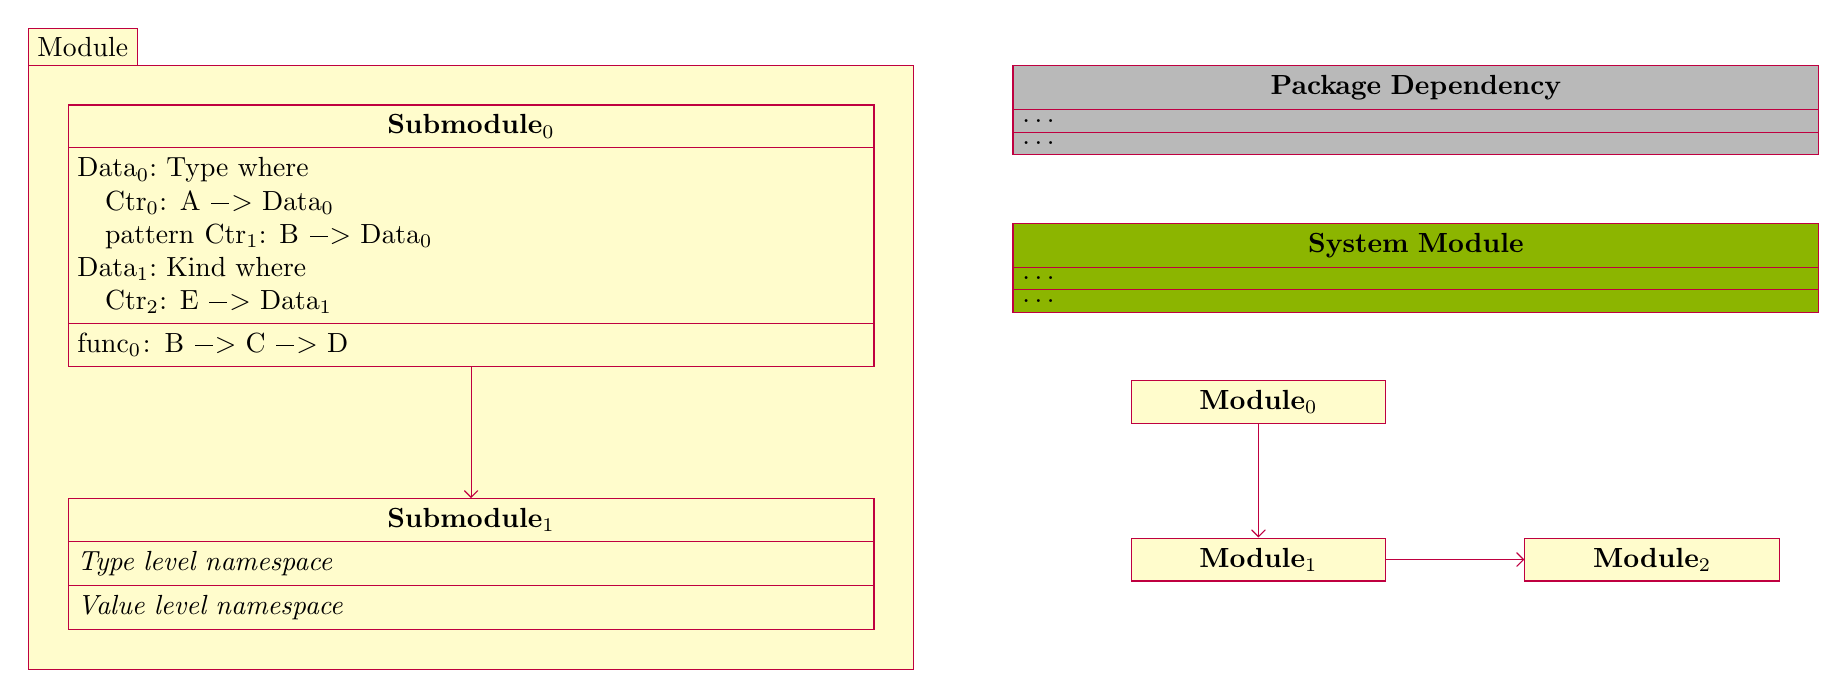
\begin{tikzpicture}

  \begin{package}{Module}

    \begin{class}[text width=10cm]{Submodule$_0$}{0,0}
      \hstype{Data$_0$ : Type where}
      \hstypectr{Ctr$_0$ : A -> Data$_0$}
      \hstypectr{pattern Ctr$_1$ : B -> Data$_0$}
      \hsfunc{func$_0$ : B -> C -> D} 
      \hstype{Data$_1$ : Kind where}
      \hstypectr{Ctr$_2$ : E -> Data$_1$}
    \end{class}

    \begin{class}[text width=10cm]{Submodule$_1$}{0,-5}
      \attribute{\emph{Type level namespace}}
      \operation{\emph{Value level namespace}}
    \end{class}
    
    \draw [umlcd style, ->] (Submodule$_0$.south) -- (Submodule$_0$ |- Submodule$_1$.north); 
  \end{package}

  \begin{class}[text width=3cm]{Module$_0$}{10,-3.5}
  \end{class}

  \begin{class}[text width=3cm]{Module$_1$}{10,-5.5}
  \end{class}

  \begin{class}[text width=3cm]{Module$_2$}{15,-5.5}
  \end{class}

  \draw [umlcd style, ->] (Module$_0$.south) -- (Module$_0$ |- Module$_1$.north); 
  \draw [umlcd style, ->] (Module$_1$.east) -- (Module$_1$ -| Module$_2$.west); 

  \renewcommand{\umlfillcolor}{grey}
    \begin{class}[text width=10cm]{Package Dependency}{12,0.5}
      \hstype{$\ldots$}
      \hsfunc{$\ldots$}
    \end{class}


  \renewcommand{\umlfillcolor}{applegreen}
    \begin{class}[text width=10cm]{System Module}{12,-1.5}
      \hstype{$\ldots$}
      \hsfunc{$\ldots$}
    \end{class}

\end{tikzpicture}
}}\caption{Example of module diagram syntax}\label{fig:ModExample}
\end{figure}



\subsection{Module Hierarchy}

\begin{figure}[!ht]
\makebox[\textwidth][c]{
\scalebox{0.6}{
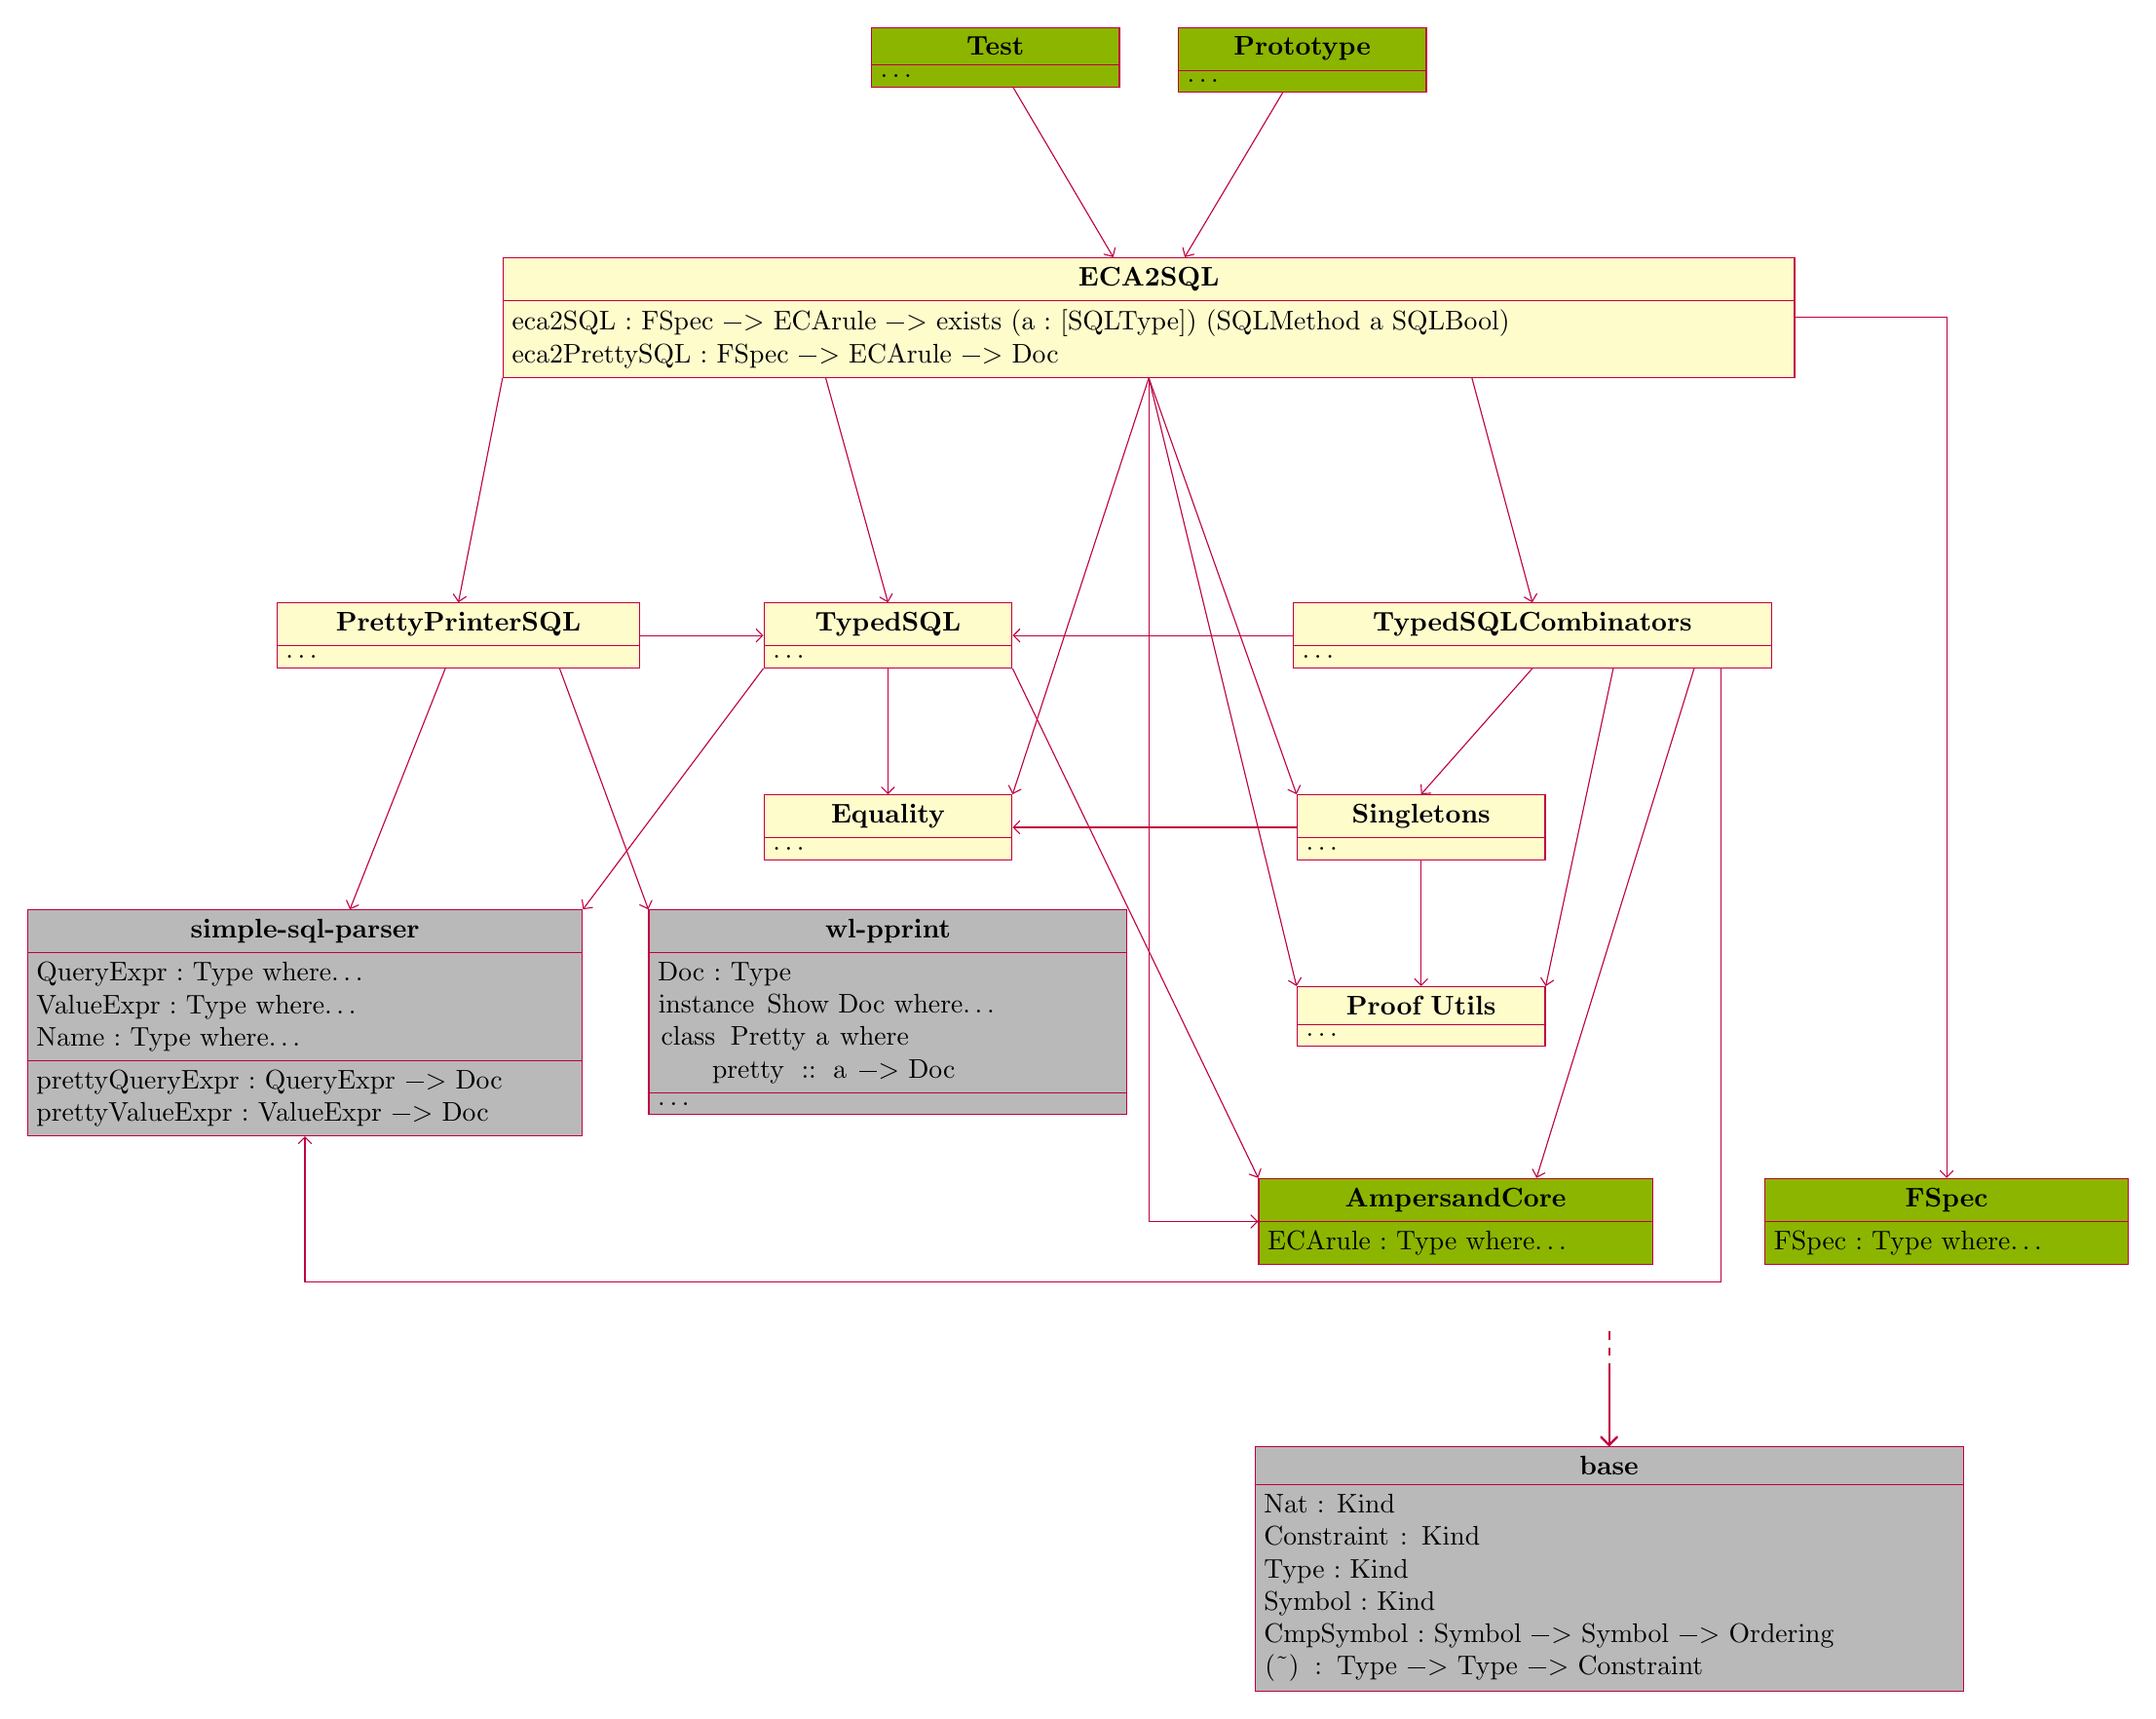
\begin{tikzpicture}
  
  %% \begin{package}{TypedSQL}
    %% fwQcGWGGF

  \begin{class}[text width=16.6cm]{ECA2SQL}{0,2}
    \hsfunc{eca2SQL : FSpec -> ECArule -> exists (a : [SQLType]) (SQLMethod a SQLBool)}
    \hsfunc{eca2PrettySQL : FSpec -> ECArule -> Doc}
      %% \hsfunc{$\ldots$}
  \end{class}

  \begin{class}[text width=3cm]{TypedSQL}{-3.4, -2.5}
      \hsfunc{$\ldots$}
  \end{class}

  \begin{class}[text width=4.5cm]{PrettyPrinterSQL}{-9, -2.5}
      \hsfunc{$\ldots$}
  \end{class}

  \begin{class}[text width=6cm]{TypedSQLCombinators}{5,-2.5}
      \hsfunc{$\ldots$}
  \end{class}


  \begin{class}[text width=3cm]{Equality}{-3.4,-5}
      \hsfunc{$\ldots$}
  \end{class}

  \begin{class}[text width=3cm]{Singletons}{3.55,-5}
      \hsfunc{$\ldots$}
  \end{class}


  %% \begin{class}[text width=3cm]{Trace}{-3.4,-13.5}
  %%     \hsfunc{$\ldots$}
  %% \end{class}

  \begin{class}[text width=3cm]{Proof Utils}{3.55,-7.5}
      \hsfunc{$\ldots$}
  \end{class}

  \renewcommand{\umlfillcolor}{grey}
  \begin{class}[text width=9cm]{base}{6,-13.5}
      \hstype{Nat : Kind} 
      \hstype{Constraint : Kind} 
      \hstype{Type : Kind} 
      \hstype{Symbol : Kind}
      \hstype{CmpSymbol : Symbol -> Symbol -> Ordering} 
      \hstype{(\~) : Type -> Type -> Constraint} 
  \end{class}

  \renewcommand{\umlfillcolor}{grey}
  \begin{class}[text width=6cm]{wl-pprint}{-3.4,-6.5}
    \hstype{Doc : Type} 
    \hstype{instance Show Doc where $\ldots$} 
    \hstype{class Pretty a where}
    \hstype[20pt]{pretty :: a -> Doc}
      \hsfunc{$\ldots$}
  \end{class}

  \renewcommand{\umlfillcolor}{grey}
  \begin{class}[text width=7cm]{simple-sql-parser}{-11,-6.5}
      \hstype{QueryExpr : Type where $\ldots$}
      \hstype{ValueExpr : Type where $\ldots$}
      \hstype{Name : Type where $\ldots$}
      \hsfunc{prettyQueryExpr : QueryExpr -> Doc} 
      \hsfunc{prettyValueExpr : ValueExpr -> Doc} 
  \end{class}


  \renewcommand{\umlfillcolor}{applegreen}
  \begin{class}[text width=4.9cm]{AmpersandCore}{4,-10}
    \hstype{ECArule : Type where $\ldots$} 
      %% \hsfunc{$\ldots$}
  \end{class}

  \renewcommand{\umlfillcolor}{applegreen}
  \begin{class}[text width=3cm]{Test}{-2,5}
      \hsfunc{$\ldots$}
  \end{class}

  \renewcommand{\umlfillcolor}{applegreen}
  \begin{class}[text width=3cm]{Prototype}{2,5}
      \hsfunc{$\ldots$}
  \end{class}

  \renewcommand{\umlfillcolor}{applegreen}
  \begin{class}[text width=4.5cm]{FSpec}{10.4,-10}
    \hstype{FSpec : Type where $\ldots$} 
      %% \hsfunc{$\ldots$}
  \end{class}

  \unidirectionalAssociation{Prototype}{}{}{ECA2SQL}
  \unidirectionalAssociation{Test}{}{}{ECA2SQL}

  \draw [umlcd style, ->] ($(ECA2SQL.south)!0.5!(ECA2SQL.south west)$) -- (TypedSQL.north); 
  \draw [umlcd style, ->] ($(ECA2SQL.south)!0.5!(ECA2SQL.south east)$) -- (TypedSQLCombinators.north); 
  \draw [umlcd style, ->] (ECA2SQL.south) -- (Equality.north east); 
  \draw [umlcd style, ->] (ECA2SQL.south) -- (Singletons.north west); 
  %% \draw [umlcd style, ->] (ECA2SQL.south) -- (Trace.north east); 
  \draw [umlcd style, ->] (ECA2SQL.south) -- (Proof Utils.north west); 
  \draw [umlcd style, ->] (ECA2SQL.south west) -- (PrettyPrinterSQL.north); 


  \node[above = 1cm of base] (basedummy)       {};
  \node[above = 1.5cm of base](basedummy2)       {};
  \draw [umlcd style, ->, thick] (basedummy) -- (base); 
  \draw [umlcd style dashed line, -, thick] (basedummy2) -- (base); 

  \draw [umlcd style, ->] (Singletons.south) -- (Proof Utils.north); 
  %% \draw [umlcd style, ->] (Singletons.west) -- (Trace.east); 
  \draw [umlcd style, ->] (TypedSQL.south) -- (Equality.north); 
  %% \draw [umlcd style, ->] (Equality.south) -- (Trace.north); 
  \draw [umlcd style, ->] (TypedSQLCombinators.west) -- (TypedSQL.east); 
  \draw [umlcd style, ->] (Singletons.west) -- (Equality.east); 
  %% \draw [umlcd style, ->] (Proof Utils.south west) -- (Trace.south east); 
  \draw [umlcd style, ->] (TypedSQL.south east) -- (AmpersandCore.north west); 

  \draw [umlcd style, ->] ([xshift=60pt]TypedSQLCombinators.south) -- ([xshift=30pt]AmpersandCore.north); 
  \draw [umlcd style, ->] (TypedSQLCombinators.south) -- (Singletons.north); 
  \draw [umlcd style, ->] ([xshift=30pt]TypedSQLCombinators.south) -- (Proof Utils.north east); 


  \draw [umlcd style, ->] ([xshift=-30pt]PrettyPrinterSQL.south east) -- (wl-pprint.north west); 
  %% \draw [umlcd style, ->] (PrettyPrinterSQL.south east) -- (Trace.west); 
  \draw [umlcd style, ->] (PrettyPrinterSQL.east) -- (TypedSQL.west); 

  %% \node[above = 1cm of Trace] (tracedummy)       {};
  %% \node[above = 1.5cm of Trace](tracedummy2)       {};
  %% \draw [umlcd style, ->, thick] (tracedummy) -- (Trace); 
  %% \draw [umlcd style dashed line, -, thick] (tracedummy2) -- (Trace); 
  
  \draw [umlcd style, ->] (TypedSQL.south west) -- (simple-sql-parser.north east); 

  \draw  [umlcd style, ->, fill opacity=0]  ([xshift=70pt]TypedSQLCombinators.south) --++ (0cm,-8cm) -| (simple-sql-parser.south);


  \draw[umlcd style ,->, fill opacity=0] (ECA2SQL.east) -| node[above , sloped , black]{} (FSpec.north);

  \draw[umlcd style ,->, fill opacity=0] (ECA2SQL.south) |- node[above , sloped , black]{} (AmpersandCore.west);

  \unidirectionalAssociation{PrettyPrinterSQL}{}{}{simple-sql-parser}

\end{tikzpicture}
}}\caption{Module diagram for EFA as a whole} \label{fig:efaMod}
\end{figure}


\Oldsubsubsection{Coarse module hierarchy}

This section contains a hierarchal breakdown of each module, as well as a brief
explanation of each modules' elements. 

The module heiarchy of EFA as a whole is given in figure~\ref{fig:efaMod}.
Note that every module which is part of EFA depends on the
Haskell ``base'' package (which is the core libraries of Haskell). Also note
that for the ``base'' package, we only include primitive definitions (i.e. those
not defined in real Haskell) which may be difficult to track down in the
documentation. The kinds ``Nat'' and ``Symbol'' correspond to type level natural
number and string literals, respectively, whose detailed semantics can be found
in the GHC user guide~\cite{ghcUserGuide}. All other features of GHC are
detailed in the user guide as well.

The primary interface to EFA is the function ``eca2PrettySQL'', which takes an
FSpec (the abstract syntax of Ampersand) and an ECA rule, and returns the pretty
printed SQL code for that rule. Also note that while the dependencies within EFA
modules is relatively complex, they depend on the rest of the Ampersand system
in a simple manner. The modules ``Test'' and ``Prototype'' implement the testing
framework and the prototype generation, respectively; these modules depend
directly on only one module from EFA, namely ``ECA2SQL''. Similarly, the
majority of EFA itself does not depend directly on Ampersand modules outside of
EFA. This makes EFA very resilient to changes in the core Ampersand system; in
order to update EFA to work with a modification to Ampersand, only one EFA
module -- ECA2SQL -- will generally need to be modified. 

All functions named in the module hierarchy are total - they do not throw
exceptions, or produce unhandled errors or infinite loops. Therefore, no
additional information past the type of the function is required to deduce the
inputs and ouputs of the function -- they are precisely the inputs and outputs
of the type.


\FloatBarrier

\begin{figure}[!ht]
\makebox[\textwidth][c]{
\scalebox{0.6}{
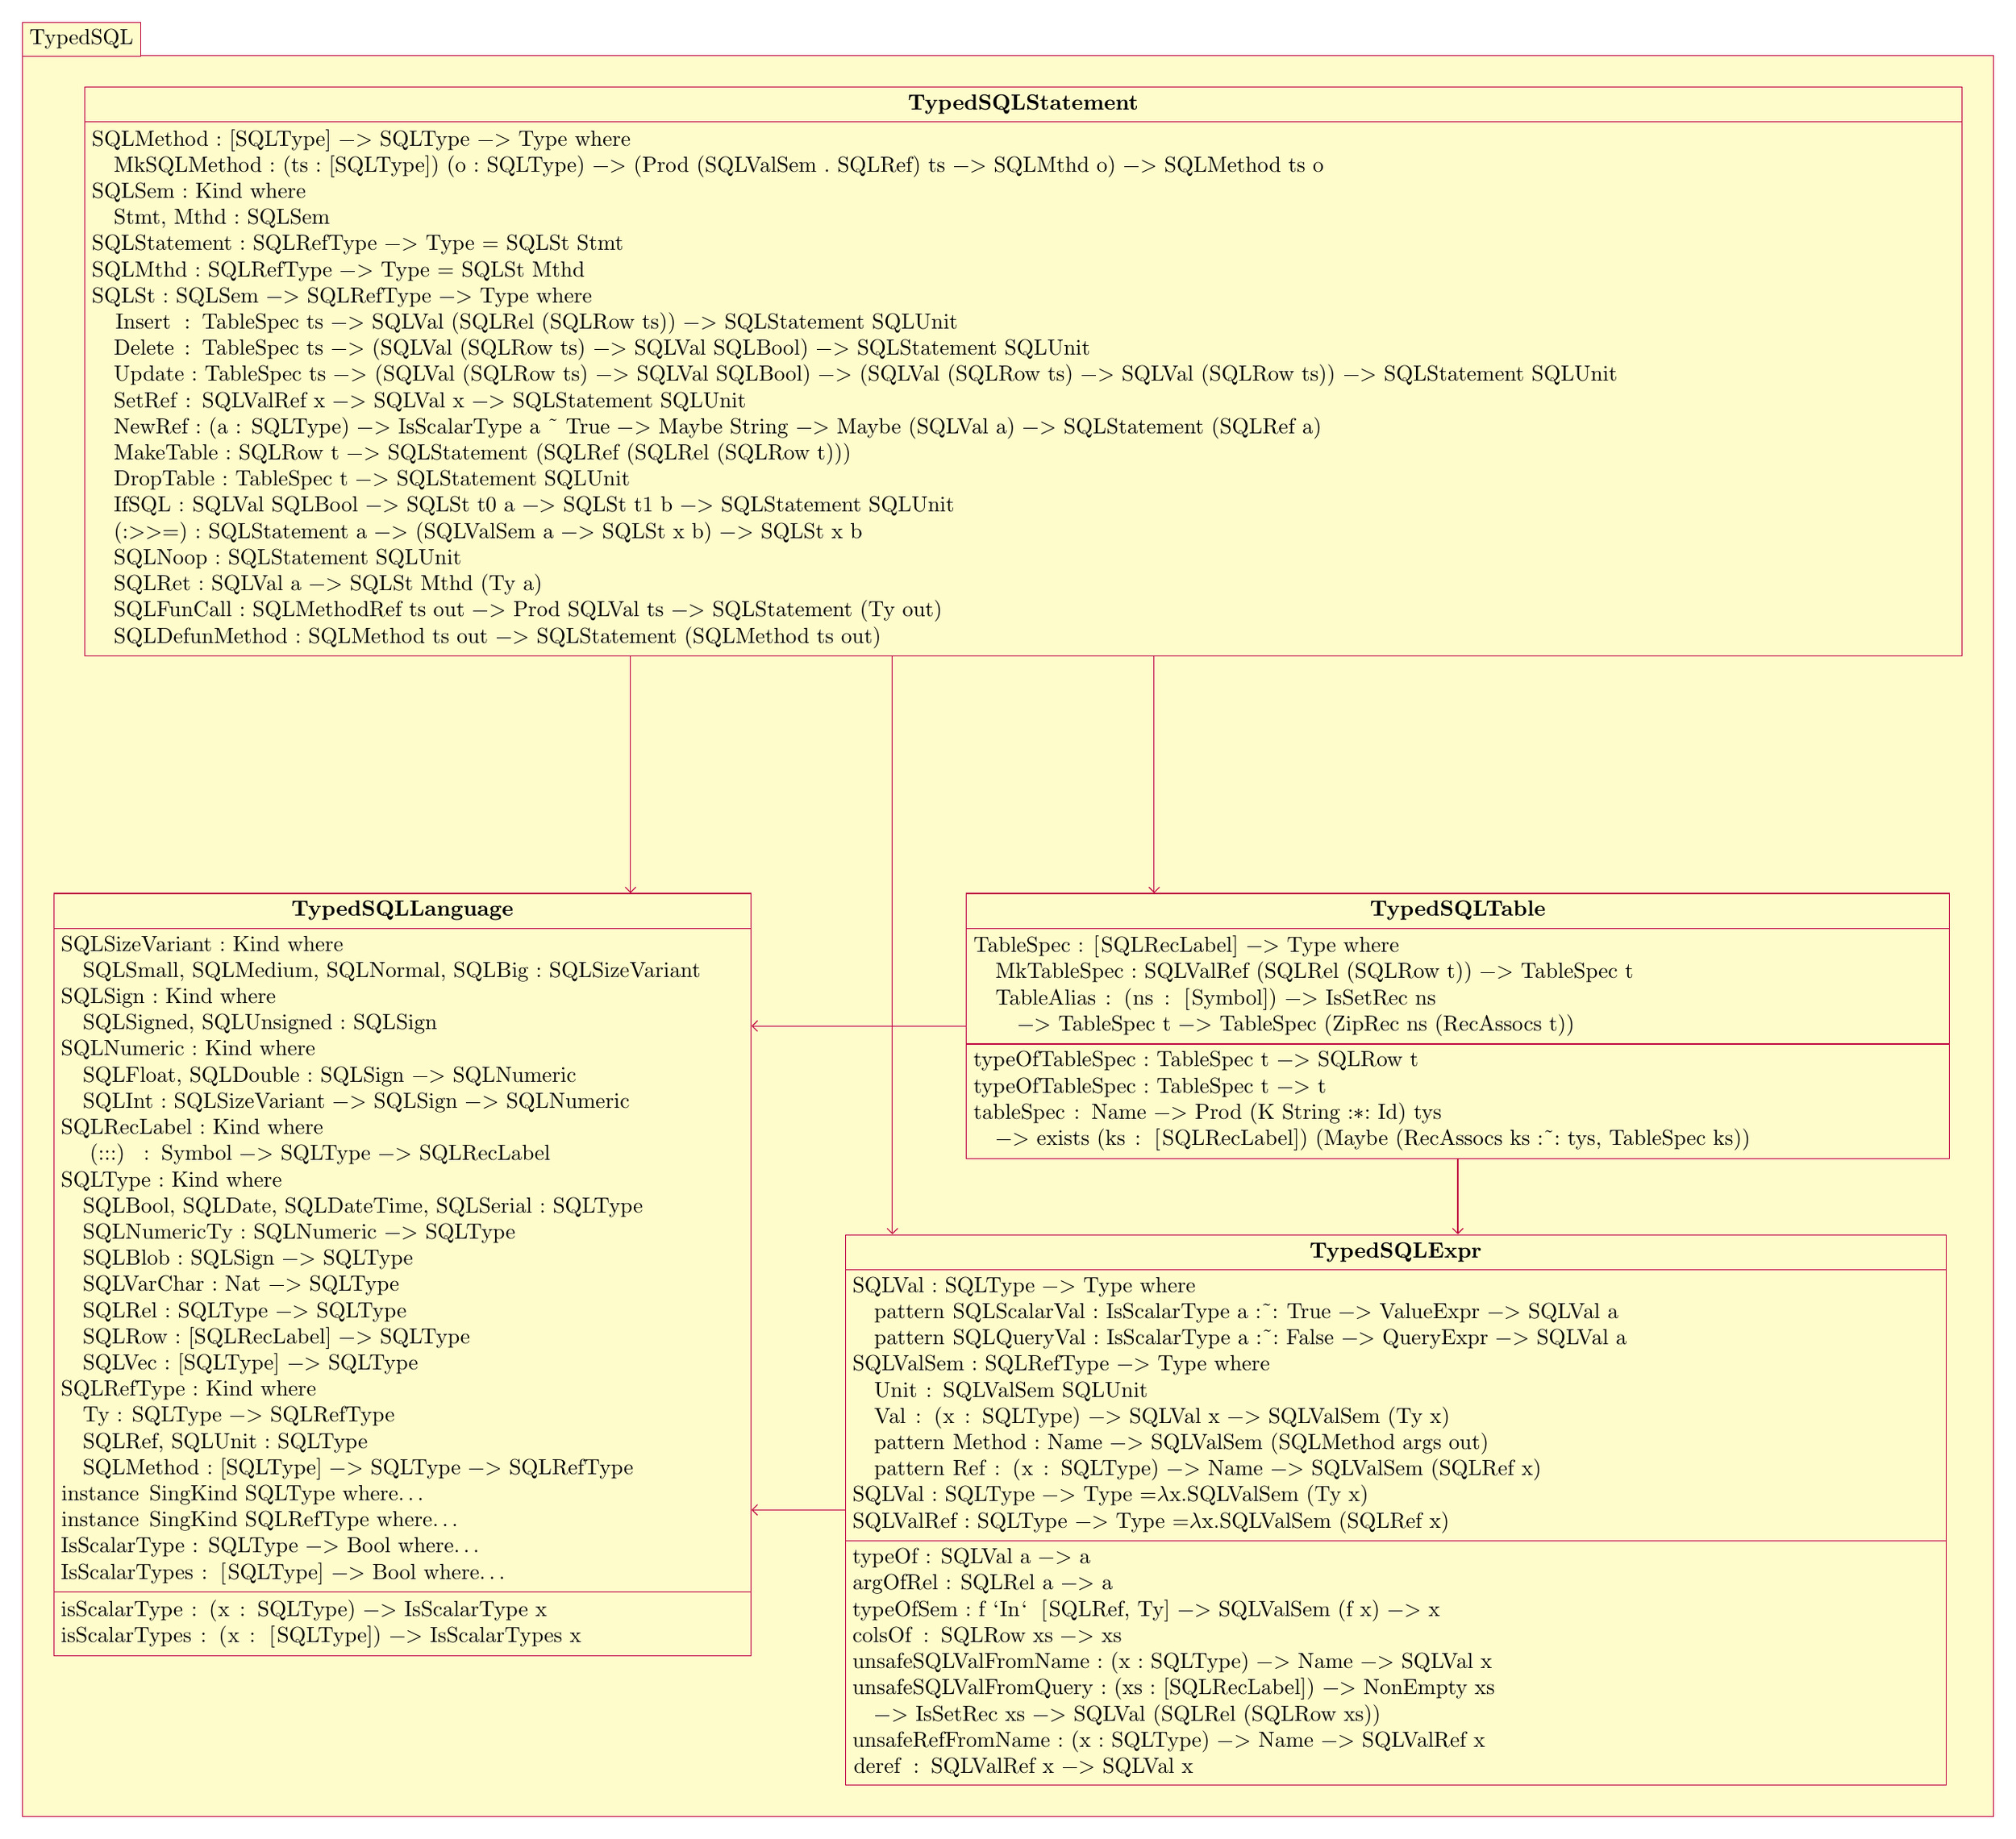
\begin{tikzpicture}

  \begin{package}{TypedSQL}

  \begin{class}[text width=30cm]{TypedSQLStatement}{10,18}
    \hstype{SQLMethod : [SQLType] -> SQLType -> Type where}
    \hstypectr{MkSQLMethod : (ts : [SQLType]) (o : SQLType) -> (Prod (SQLValSem . SQLRef) ts -> SQLMthd o) -> SQLMethod ts o}
    %% \hstype[20pt]{-> (Prod (SQLValSem . SQLRef) ts -> SQLMthd o) -> SQLMethod ts o}
     
    \hstype{SQLSem : Kind where}
    \hstypectr{Stmt, Mthd : SQLSem}

    \hstype{SQLStatement : SQLRefType -> Type = SQLSt Stmt}
    \hstype{SQLMthd : SQLRefType -> Type = SQLSt Mthd}

    \hstype{SQLSt : SQLSem -> SQLRefType -> Type where} 
    \hstypectr{Insert : TableSpec ts -> SQLVal (SQLRel (SQLRow ts)) -> SQLStatement SQLUnit}
    \hstypectr{Delete : TableSpec ts -> (SQLVal (SQLRow ts) -> SQLVal SQLBool) -> SQLStatement SQLUnit}
    \hstypectr{Update : TableSpec ts -> (SQLVal (SQLRow ts) -> SQLVal SQLBool) -> (SQLVal (SQLRow ts) -> SQLVal (SQLRow ts)) -> SQLStatement SQLUnit}
    \hstypectr{SetRef : SQLValRef x -> SQLVal x -> SQLStatement SQLUnit}
    \hstypectr{NewRef : (a : SQLType) -> IsScalarType a \~ True -> Maybe String -> Maybe (SQLVal a) -> SQLStatement (SQLRef a)}
    \hstypectr{MakeTable : SQLRow t -> SQLStatement (SQLRef (SQLRel (SQLRow t)))}
    \hstypectr{DropTable : TableSpec t -> SQLStatement SQLUnit}
    \hstypectr{IfSQL : SQLVal SQLBool -> SQLSt t0 a -> SQLSt t1 b -> SQLStatement SQLUnit}
    \hstypectr{(:>>=) : SQLStatement a -> (SQLValSem a -> SQLSt x b) -> SQLSt x b}
    \hstypectr{SQLNoop : SQLStatement SQLUnit}
    \hstypectr{SQLRet : SQLVal a -> SQLSt Mthd (Ty a)}
    \hstypectr{SQLFunCall : SQLMethodRef ts out -> Prod SQLVal ts -> SQLStatement (Ty out)}
    \hstypectr{SQLDefunMethod : SQLMethod ts out -> SQLStatement (SQLMethod ts out)}
  \end{class}


  \begin{class}[text width=11cm]{TypedSQLLanguage}{0,5}   
    \hstype{SQLSizeVariant : Kind where}
    \hstypectr{SQLSmall, SQLMedium, SQLNormal, SQLBig : SQLSizeVariant}

    \hstype{SQLSign : Kind where}
    \hstypectr{SQLSigned, SQLUnsigned : SQLSign}

    \hstype{SQLNumeric : Kind where}
    \hstypectr{SQLFloat, SQLDouble : SQLSign -> SQLNumeric}
    \hstypectr{SQLInt : SQLSizeVariant -> SQLSign -> SQLNumeric}

    \hstype{SQLRecLabel : Kind where}
    \hstypectr{(:::) : Symbol -> SQLType -> SQLRecLabel}

    \hstype{SQLType : Kind where}
    \hstypectr{SQLBool, SQLDate, SQLDateTime, SQLSerial : SQLType}
    \hstypectr{SQLNumericTy : SQLNumeric -> SQLType}
    \hstypectr{SQLBlob : SQLSign -> SQLType}
    \hstypectr{SQLVarChar : Nat -> SQLType}
    \hstypectr{SQLRel : SQLType -> SQLType}
    \hstypectr{SQLRow : [SQLRecLabel] -> SQLType}
    \hstypectr{SQLVec : [SQLType] -> SQLType}

    \hstype{SQLRefType : Kind where}
    \hstypectr{Ty : SQLType -> SQLRefType}
    \hstypectr{SQLRef, SQLUnit : SQLType}
    \hstypectr{SQLMethod : [SQLType] -> SQLType -> SQLRefType}

    \hstype{instance SingKind SQLType where $\ldots$}
    \hstype{instance SingKind SQLRefType where $\ldots$}

    \hstype{IsScalarType : SQLType -> Bool where $\ldots$}
    \hstype{IsScalarTypes : [SQLType] -> Bool where $\ldots$}

    \hsfunc{isScalarType : (x : SQLType) -> IsScalarType x}
    \hsfunc{isScalarTypes : (x : [SQLType]) -> IsScalarTypes x}
  \end{class}


  \begin{class}[text width=17.5cm]{TypedSQLExpr}{16,-0.5}
    \hstype{SQLVal : SQLType -> Type where}
    \hstypectr{pattern SQLScalarVal : IsScalarType a :\~: True -> ValueExpr -> SQLVal a}
    \hstypectr{pattern SQLQueryVal  : IsScalarType a :\~: False -> QueryExpr -> SQLVal a}

    \hsfunc{typeOf : SQLVal a -> a}
    \hsfunc{argOfRel : SQLRel a -> a} 

    \hstype{SQLValSem : SQLRefType -> Type where}
    \hstypectr{Unit : SQLValSem SQLUnit}
    \hstypectr{Val : (x : SQLType) -> SQLVal x -> SQLValSem (Ty x)}
    \hstypectr{pattern Method : Name -> SQLValSem (SQLMethod args out)}
    \hstypectr{pattern Ref : (x : SQLType) -> Name -> SQLValSem (SQLRef x)}
    
    \hstype{SQLVal : SQLType -> Type = $\lambda$ x $.$ SQLValSem (Ty x)}
    \hstype{SQLValRef : SQLType -> Type = $\lambda$ x $.$ SQLValSem (SQLRef x)}

    \hsfunc{typeOfSem : f `In` [SQLRef, Ty] -> SQLValSem (f x) -> x}
 
    \hsfunc{colsOf : SQLRow xs -> xs}

    \hsfunc{unsafeSQLValFromName : (x : SQLType) -> Name -> SQLVal x}
    \hsfunc{unsafeSQLValFromQuery : (xs : [SQLRecLabel]) -> NonEmpty xs}
    \hsfunc[10pt]{ -> IsSetRec xs -> SQLVal (SQLRel (SQLRow xs))}
    \hsfunc{unsafeRefFromName : (x : SQLType) -> Name -> SQLValRef x}

    \hsfunc{deref : SQLValRef x -> SQLVal x}   
  \end{class}


  \begin{class}[text width=15.6cm]{TypedSQLTable}{17,5}
    \hstype{TableSpec : [SQLRecLabel] -> Type where}
    \hstypectr{MkTableSpec : SQLValRef (SQLRel (SQLRow t))  -> TableSpec t}
    \hstypectr{TableAlias : (ns : [Symbol]) -> IsSetRec ns }
    \hstype[20pt]{-> TableSpec t -> TableSpec (ZipRec ns (RecAssocs t))}

    \hsfunc{typeOfTableSpec : TableSpec t -> SQLRow t}
    \hsfunc{typeOfTableSpec : TableSpec t -> t}

    \hsfunc{tableSpec : Name -> Prod (K String :*: Id) tys}
    \hsfunc[10pt]{ -> exists (ks : [SQLRecLabel]) (Maybe (RecAssocs ks :\~: tys, TableSpec ks))}

  \end{class}

  \draw [umlcd style, ->] ([xshift=-60pt]TypedSQLStatement.south) -- ([xshift=-60pt]TypedSQLStatement |- TypedSQLExpr.north); 
  \draw [umlcd style, ->] ([xshift=60pt]TypedSQLStatement.south) -- ([xshift=60pt]TypedSQLStatement |- TypedSQLTable.north); 
  \draw [umlcd style, ->] ([xshift=-180pt]TypedSQLStatement.south) -- ([xshift=-180pt]TypedSQLStatement |- TypedSQLLanguage.north); 
  

  \draw [umlcd style, ->] (TypedSQLTable.south) -- (TypedSQLTable |- TypedSQLExpr.north); 
  \draw [umlcd style, ->] (TypedSQLTable.west) -- (TypedSQLTable -| TypedSQLLanguage.east); 
  \draw [umlcd style, ->] (TypedSQLExpr.west) -- (TypedSQLExpr -| TypedSQLLanguage.east);

  \end{package}

\end{tikzpicture}
}}\caption{Module diagram for TypedSQL} \label{fig:typedSQL}
\end{figure}


\Oldsubsubsection{TypedSQL}

The module hierarchy for the TypedSQL module is shown in
figure~\ref{fig:typedSQL}. The submodules of TypedSQL are quite large, however,
the majority of the definitions within are type and kind definitions, which correspond 
precisely to entities defined by MySQL. The only exception is SQLRel, which distinguishes
relations from scalar types - MySQL does not make this distinguishment. Only a few
helper functions are defined in these modules -- namely, only things which form
the core interface to TypedSQL and in particular, SQLStatement. These functions
cannot be defined outside of the module, usually because they use an abstract
constructor. By making the core interface to TypedSQL very small, maintaining 
the TypedSQL language definition separately from the implementation of 
EFA is simplified. All of the data types in TypedSQL are correct by 
construction, with the exception of the functions explicitly labeled ``unsafe''.
These functions (unsafeSQLValFromName, unsafeSQLValFromQuery, and unsafeRefFromName)
are required only when implementing a new SQL primitive on top of the SQL
language - they are not intended for regular use. 

The TypedSQLLanguage module models the SQL type language in Haskell with a
series of kind declarations. The language being modeled is only a subset of the
SQL type language, corresponding approximately to the subset which the core
Ampersand system already uses. The meaning of each Haskell type corresponds
exactly to the appropriate MySQL type, which are detailed in the MySQL
manual~\cite{mySQLman}. Similarly, the constructors of SQLSt all correspond
to different varieties of SQL statements -- for the majority of constructors,
there is a one-to-one correspondence between the semantics of the constructor,
and the semantics of the SQL statement with the same name. The exceptions 
are: 

\begin{description}
\item[\texttt{SQLNoop}] MySQL does not have a primitive no-op statement
\item[\texttt{SQLDefunMethod}]  MySQL does not allow defining procedures within procedures; 
  this constructor denotes that a method ``defined'' within another statement must 
  first be loaded as a MySQL Stored Procedure ~\cite{mySQLman}.
\item[\texttt{:>>=}] This constructor corresponds to sequencing statements. This constructor
  embeds scope checking of MySQL statements in the Haskell compiler -- ill-formed statements
  containing variables which are not defined (i.e. not in scope) will be rejected by the Haskell
  compiler. 
\end{description}

The SQLSt data type also distinguishes between two varieties of statements:
SQLStatement and SQLMthd. The former is the type of regular statements, while
the latter is the type of ``almost'' complete methods - methods whose formal
parameters have not yet been bound. This is done in order to statically
guarantee that a SQL method always returns a value. Due to the type of
\lstinline{:>>=}, this also rules out SQL programs which contain dead code -- no
code can follow SQLRet, which is always guaranteed to return from the function.
While this does rule out some valid programs (for example, an if statement in
which both branches end with a return, but there is no return following the if
statment, will be rejected), these programs can be written in an equivalent
way in our language without any loss of generality.

\begin{figure}[!ht]
\makebox[\textwidth][c]{
\scalebox{0.6}{
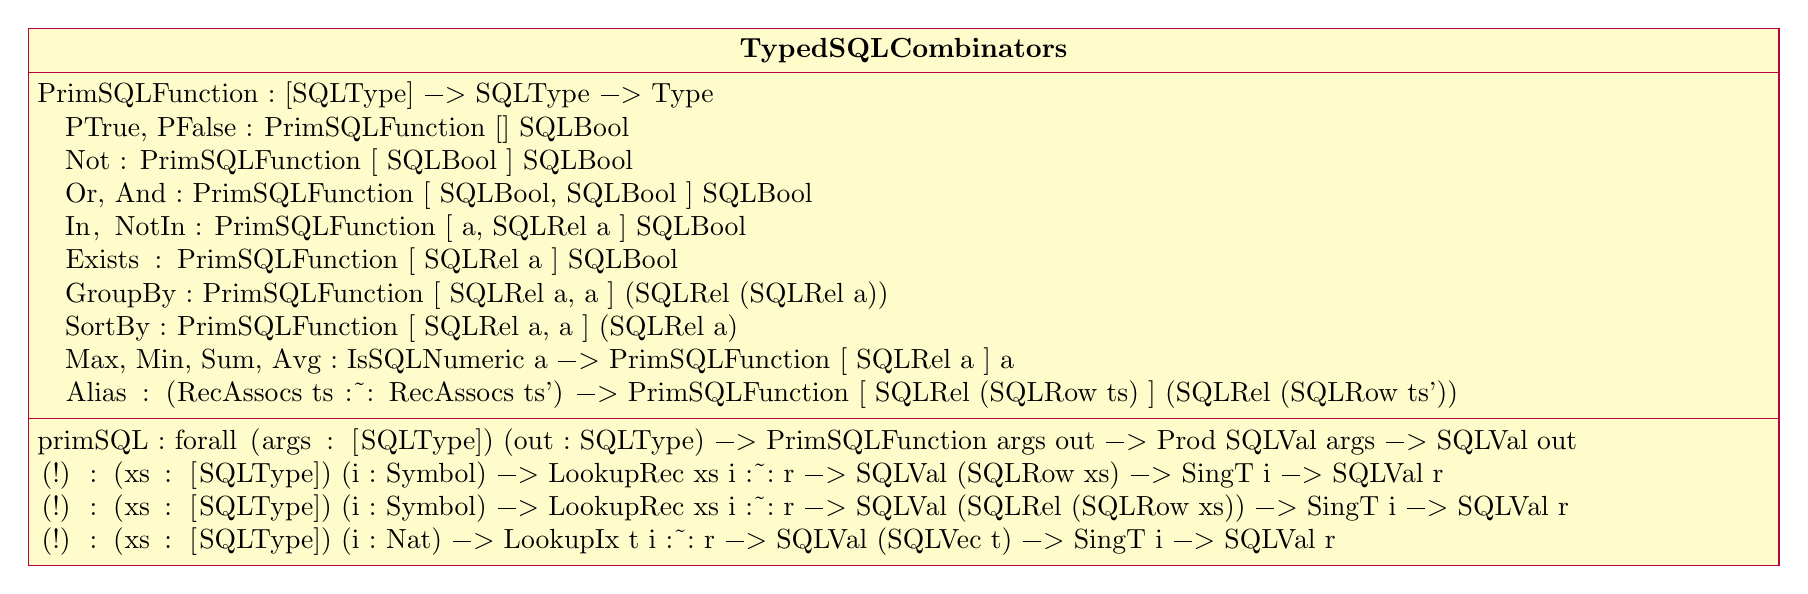
\begin{tikzpicture}
  
  %% \begin{package}{TypedSQL}
    
  \begin{class}[text width=22cm]{TypedSQLCombinators}{17,5}
    \hstype{PrimSQLFunction : [SQLType] -> SQLType -> Type}
    \hstypectr{PTrue, PFalse : PrimSQLFunction [] SQLBool}
    \hstypectr{Not : PrimSQLFunction [ SQLBool ] SQLBool}
    \hstypectr{Or, And : PrimSQLFunction [ SQLBool, SQLBool ] SQLBool}
    \hstypectr{In, NotIn : PrimSQLFunction [ a, SQLRel a ] SQLBool}
    \hstypectr{Exists : PrimSQLFunction [ SQLRel a ] SQLBool}
    \hstypectr{GroupBy : PrimSQLFunction [ SQLRel a, a ] (SQLRel (SQLRel a))}
    \hstypectr{SortBy  : PrimSQLFunction [ SQLRel a, a ] (SQLRel a)}
    \hstypectr{Max, Min, Sum, Avg : IsSQLNumeric a -> PrimSQLFunction [ SQLRel a ] a }
    \hstypectr{Alias : (RecAssocs ts :~: RecAssocs ts') -> PrimSQLFunction [ SQLRel (SQLRow ts) ] (SQLRel (SQLRow ts'))}

    \hsfunc{primSQL : forall (args : [SQLType]) (out : SQLType) -> PrimSQLFunction args out -> Prod SQLVal args -> SQLVal out}

    \hsfunc{(!) : (xs : [SQLType]) (i : Symbol) -> LookupRec xs i :\~: r -> SQLVal (SQLRow xs) -> SingT i -> SQLVal r}
    \hsfunc{(!) : (xs : [SQLType]) (i : Symbol) -> LookupRec xs i :\~: r -> SQLVal (SQLRel (SQLRow xs)) -> SingT i -> SQLVal r}
    \hsfunc{(!) : (xs : [SQLType]) (i : Nat) -> LookupIx t i :\~: r -> SQLVal (SQLVec t) -> SingT i -> SQLVal r}
   
    
  \end{class}

  %% \end{package}

\end{tikzpicture}
}}\caption{Module diagram for TypedSQLCombinators} \label{fig:typedSQLComb}
\end{figure}

\Oldsubsubsection{TypedSQLCombinators}

The module TypedSQLCombinators, whose members are given in figure~\ref{fig:typedSQLComb},
implements a subset of primitive SQL functions on top of the TypedSQL expression type. 
The data type PrimSQLFunction encodes the specification of each function; the type
and semantics of each function is that of the corresponding function in MySQL (refer to
the MySQL manual ~\cite{mySQLman} for details on each function). The only exception
is the ``Alias'' function, which is a primitive syntactic constructor (not a named entity)
in MySQL - rows can be aliased with a select statement. Aliasing a row means to change
the name of each association in the row, but not the shape of the row (i.e. the types of
each element of the row, as well as their ordering). The single function ``primSQL''
implements all of the primitive SQL functions. It takes as an argument a specification
of the primitive function, a tuple of arguments of the correspond types, and returns
a SQL value, again of the corresponding type. 



\begin{figure}[!ht]
\makebox[\textwidth][c]{
\scalebox{0.6}{
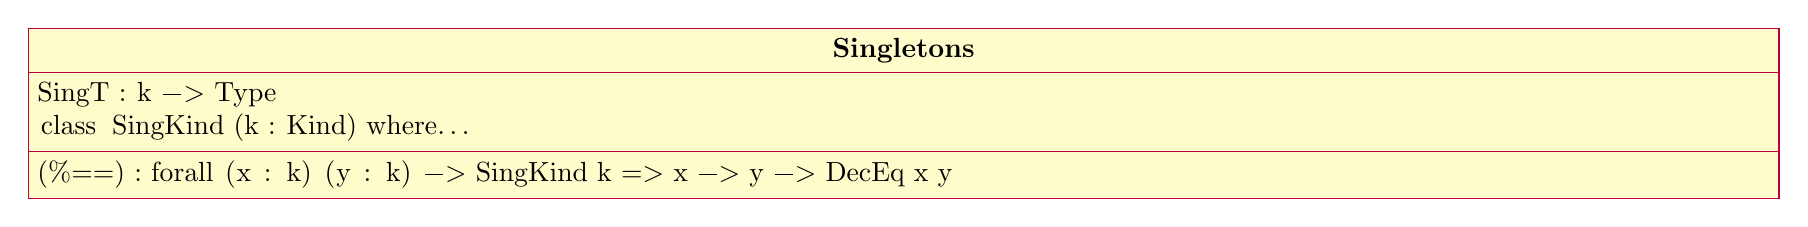
\begin{tikzpicture}
    
  \begin{class}[text width=22cm]{Singletons}{17,5}
    \hstype{SingT : k -> Type} 
    \hstype{class SingKind (k : Kind) where $\ldots$} 
    \hsfunc{(\%==) : forall (x : k) (y : k) -> SingKind k => x -> y -> DecEq x y}

  \end{class}

\end{tikzpicture}
}}\caption{Module diagram for Singletons} \label{fig:singletons}
\end{figure}

\begin{figure}[!ht]
\makebox[\textwidth][c]{
\scalebox{0.6}{
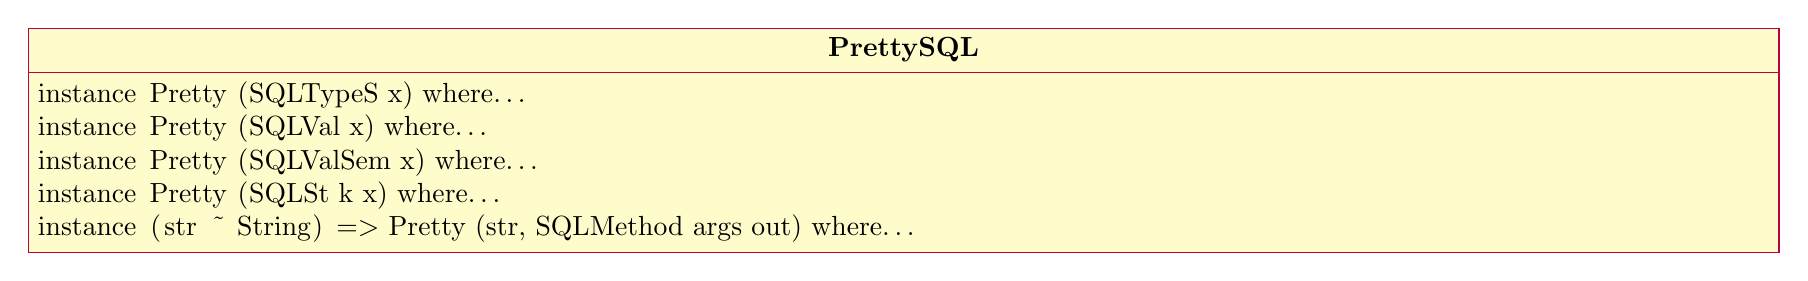
\begin{tikzpicture}
    
  \begin{class}[text width=22cm]{PrettySQL}{17,5}

    \hstype{instance Pretty (SQLTypeS x) $\,\,$ where $\ldots$}
    \hstype{instance Pretty (SQLVal x)  $\,\,$ where $\ldots$}
    \hstype{instance Pretty (SQLValSem x)  $\,\,$ where $\ldots$}
    \hstype{instance Pretty (SQLSt k x)  $\,\,$ where $\ldots$}
    \hstype{instance (str \~ String) => Pretty (str, SQLMethod args out)  $\,\,$ where $\ldots$}

  \end{class}

\end{tikzpicture}
}}\caption{Module diagram for PrettySQL} \label{fig:prettySQL}
\end{figure}



\begin{figure}[!ht]
\makebox[\textwidth][c]{
\scalebox{0.6}{
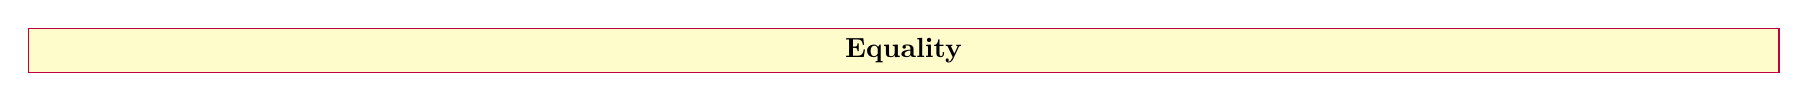
\begin{tikzpicture}
    
  \begin{class}[text width=22cm]{Equality}{17,5}
    

  \end{class}

\end{tikzpicture}
}}\caption{Module diagram for Equality} \label{fig:equality}
\end{figure}


\Oldsubsubsection{PrettySQL}

The module PrettySQL defines pretty printers for each of the types
corresponding to SQL entities, including SQL types, SQL values, SQL references
and methods, and SQL statements. These pretty printers produce a value of
type Doc (which comes from the wl-pprint package), which is like a string
, but contains the layout and indentation of all lines of the document,
allowing for easy composition of Doc values into larger documents, without
worrying about layout. The SQL entities are pretty printed in a human
readable format, complete with SQL comments which indicate the origin
and motive of generated code. 



\begin{figure}[!ht]
\makebox[\textwidth][c]{
\scalebox{0.6}{
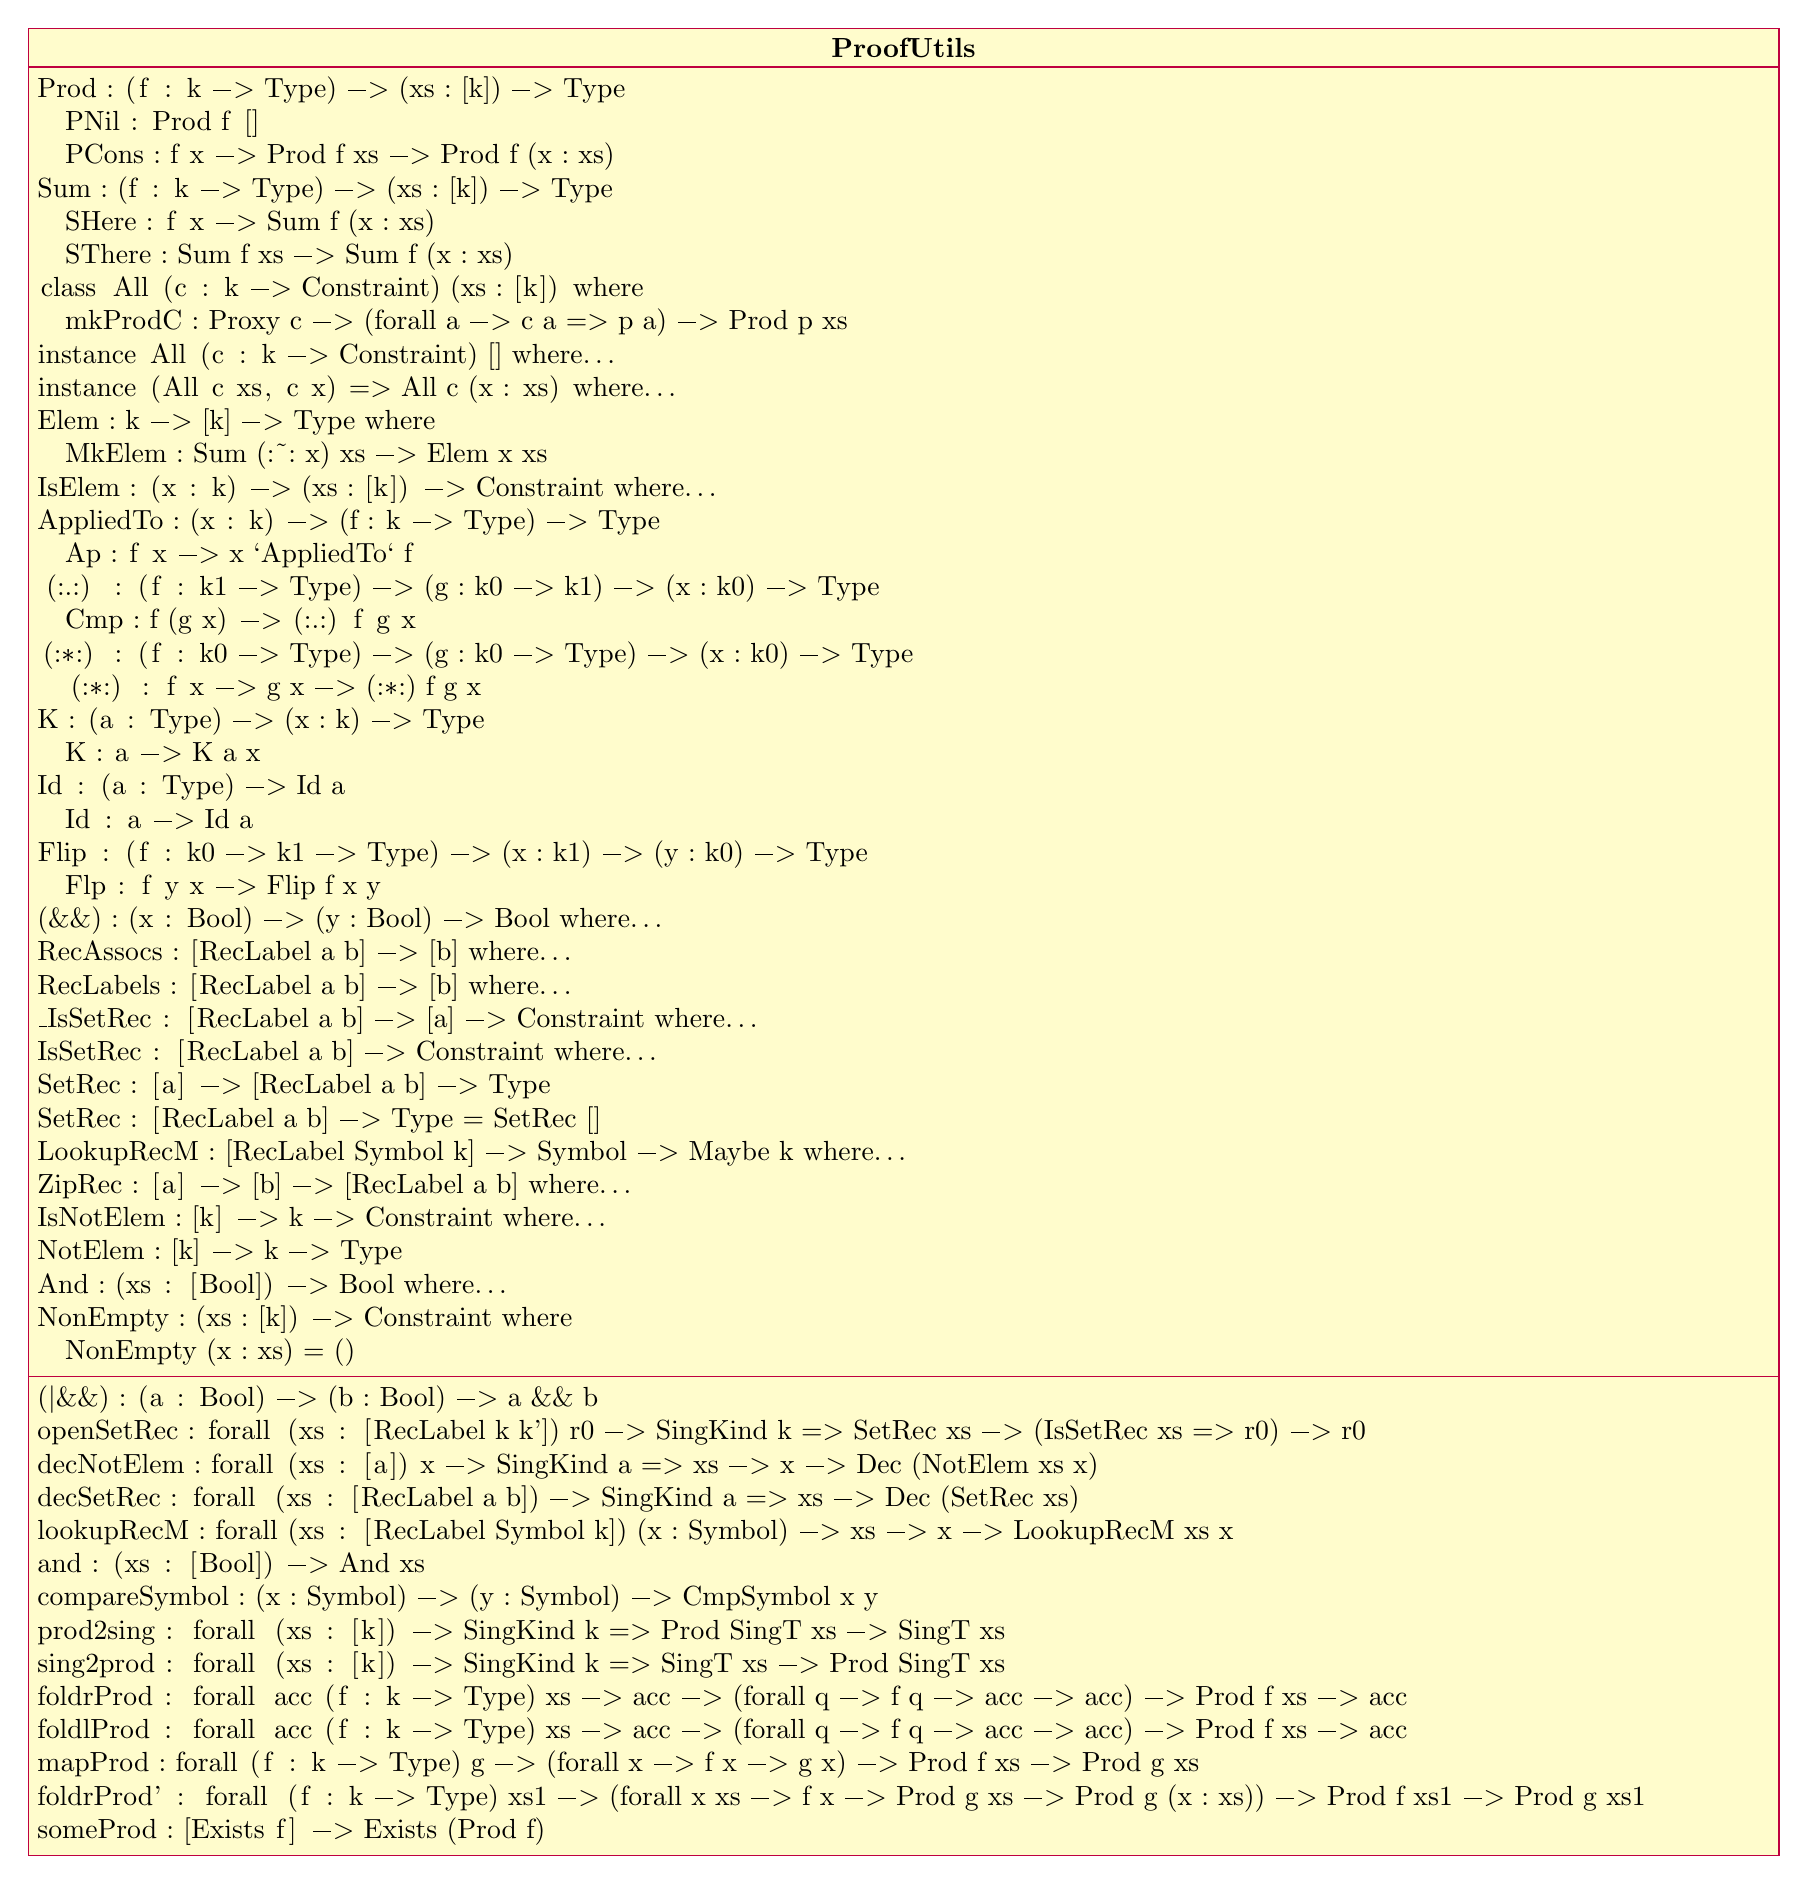
\begin{tikzpicture}
    
  \begin{class}[text width=22cm]{ProofUtils}{17,5}

   \hstype{Prod : (f : k -> Type) -> (xs : [k]) -> Type} 
   \hstypectr{PNil : Prod f []}
   \hstypectr{PCons : f x -> Prod f xs -> Prod f (x : xs)}
   
   \hstype{Sum : (f : k -> Type) -> (xs : [k]) -> Type}  
   \hstypectr{SHere : f x -> Sum f (x : xs)}
   \hstypectr{SThere : Sum f xs -> Sum f (x : xs)}

   
   \hstype{class All (c : k -> Constraint) (xs : [k]) where}
   \hstypectr{mkProdC : Proxy c -> (forall a -> c a => p a) -> Prod p xs}
   
   \hstype{instance All (c : k -> Constraint) [] where $\ldots$}
   \hstype{instance (All c xs, c x) => All c (x : xs) where $\ldots$}

   \hstype{Elem : k -> [k] -> Type where}
   \hstypectr{MkElem : Sum (:\~: x) xs -> Elem x xs} 

   \hstype{IsElem : (x : k) -> (xs : [k]) -> Constraint where $\ldots$} 
   \hstype{AppliedTo : (x : k) -> (f : k -> Type) -> Type}
   \hstypectr{Ap : f x -> x `AppliedTo` f}
   
   \hstype{(:.:) : (f : k1 -> Type) -> (g : k0 -> k1) -> (x : k0) -> Type}
   \hstypectr{Cmp : f (g x) -> (:.:) f g x} 

   \hstype{(:*:) : (f : k0 -> Type) -> (g : k0 -> Type) -> (x : k0) -> Type} 
   \hstypectr{(:*:) : f x -> g x -> (:*:) f g x} 
   \hstype{K : (a : Type) -> (x : k) -> Type} 
   \hstypectr{K : a -> K a x} 
   \hstype{Id : (a : Type) -> Id a}
   \hstypectr{Id : a -> Id a} 

   \hstype{Flip : (f : k0 -> k1 -> Type) -> (x : k1) -> (y : k0) -> Type} 
   \hstypectr{Flp : f y x -> Flip f x y} 

   \hstype{(&&) : (x : Bool) -> (y : Bool) -> Bool where $\ldots$} 
   
   \operation{\lstinline[mathescape]{(|&&) : (a : Bool) -> (b : Bool) -> a && b}}

   \hstype{RecAssocs : [RecLabel a b] -> [b] where $\ldots$} 
   \hstype{RecLabels : [RecLabel a b] -> [b] where $\ldots$} 
   
   \hstype{IsSetRec\_ : [RecLabel a b] -> [a] -> Constraint where $\ldots$} 
   
   \hstype{IsSetRec : [RecLabel a b] -> Constraint where $\ldots$} 
   \hstype{SetRec\_ : [a] -> [RecLabel a b] -> Type} 
   \hstype{SetRec : [RecLabel a b] -> Type = SetRec\_ []} 
   
   
   \hsfunc{openSetRec : forall (xs : [RecLabel k k']) $\,\,$r0 -> SingKind k => SetRec xs -> (IsSetRec xs => r0) -> r0}
   
   \hsfunc{decNotElem : forall (xs : [a]) $\,\,$x -> SingKind a => xs -> x -> Dec (NotElem xs x)}
   
   \hsfunc{decSetRec : forall (xs : [RecLabel a b]) -> SingKind a => xs -> Dec (SetRec xs)}
   
   \hstype{LookupRecM : [RecLabel Symbol k] -> Symbol -> Maybe k where $\ldots$} 
   
   \hsfunc{lookupRecM : forall (xs : [RecLabel Symbol k]) (x : Symbol) -> xs -> x -> LookupRecM xs x}
   
   \hstype{ZipRec : [a] -> [b] -> [RecLabel a b] where $\ldots$} 

   \hstype{IsNotElem :  [k] -> k -> Constraint where $\ldots$} 
   \hstype{NotElem : [k] -> k -> Type}
   
   \hstype{And : (xs : [Bool]) -> Bool where $\ldots$} 

   \hsfunc{and\_t : (xs : [Bool]) -> And xs}

   \hsfunc{compareSymbol : (x : Symbol) -> (y : Symbol) -> CmpSymbol x y}
   
   
   \hstype{NonEmpty : (xs : [k]) -> Constraint where} 
   \hstypectr{NonEmpty (x : xs) = ()} 
   
   \hsfunc{prod2sing : forall (xs : [k]) -> SingKind k => Prod SingT xs -> SingT xs} 
   \hsfunc{sing2prod : forall (xs : [k]) -> SingKind k => SingT xs -> Prod SingT xs} 
   \hsfunc{foldrProd : forall acc (f : k -> Type)$\,\,$xs -> acc -> (forall q -> f q -> acc -> acc) -> Prod f xs -> acc}
   \hsfunc{foldlProd : forall acc (f : k -> Type)$\,\,$xs -> acc -> (forall q -> f q -> acc -> acc) -> Prod f xs -> acc}
   \hsfunc{mapProd : forall (f : k -> Type)$\,\,$g -> (forall x -> f x -> g x) -> Prod f xs -> Prod g xs}
   \hsfunc{foldrProd' : forall (f : k -> Type)$\,\,$xs1 -> (forall x xs -> f x -> Prod g xs -> Prod g (x : xs)) -> Prod f xs1 -> Prod g xs1 }
   \hsfunc{someProd : [Exists f] -> Exists (Prod f)}

  \end{class}

\end{tikzpicture}
}}\caption{Module diagram for ProofUtils} \label{fig:utilsMod}
\end{figure}

\Oldsubsubsection{Proof Utils}

The ProofUtils modules, shown in figure~\ref{fig:utilsMod} provides various
utilities for proving compile time invariants, including the definitions of
various predicates used in other modules, as well as the value-level functions
which prove or disprove those predicates. Generally speaking, a predicate is a
type level function which returns either a true or false value, or has kind
\lstinline{Constraint}, in which case truth corresponds to a satisfied
constraint, while false to an unsatisfied one. Many predicates have value level
witnesses as well; these are datatypes which are inhabitted if and only if the
predicate is true.  Therefore, pattern matching on the predicate witness can be
used to recover a proof of the predicate at run time.

The function of the most imporant 
predicates and types is briefly summarized as follows. 
\begin{description}
\item[\texttt{Prod}] The type \lstinline{Prod f xs} represents the $n$-ary product of the type
  level list $xs$, with each $x \in xs$ being mapped to the type \lstinline{f x}. This 
  type is accompanied by the functions \lstinline{prod2sing, sing2prod} which convert
  between singletons and products; the functions \lstinline{foldrProd, foldlProd, foldrProd'}, 
  which are all eliminators for \lstinline{Prod} (several eliminators are needed because the 
  most general eliminator is not well typed in Haskell). 
\item[\texttt{Sum}] The same as above, but the $n$-ary sum as opposed to product. 
\item[\texttt{All}] The constraint \lstinline{All c xs} holds if and only if \lstinline{c x} holds for all $x \in xs$. 
\item[\texttt{Elem, IsElem}] \lstinline{IsElem x xs} holds precisely when $x \in xs$. \lstinline{Elem} is the witness of \lstinline{IsElem}. 
\item[\texttt{AppliedTo, Ap, :.:, Cmp, :*:, K, Id, Flip}] Categorical data types which encode
a generalized view of algebraic data types. This approach is largely standardized (and is only
replicated here to avoid incurring a large dependency) -- for more information, see~\cite{alacarte}. 
\item[\texttt{RecAssocs, RecLabels, ZipRec}] Type level functions for working with type level records. 
A record in this context is a list of types of some kind, each associated with a unique string label. 
\lstinline{RecAssocs, RecLabels} retrieve the associations and labels of a record, respecively, 
while \lstinline{ZipRec} constructs such a record from the associations and labels. It is the case
that \lstinline{ZipRec (RecAssocs x) (RecLabels x) == x} for all \lstinline{x} .
\item[\texttt{IsSetRec, SetRec}] The predicate \lstinline{IsSetRec x} holds precisely if \lstinline{x}
  is a valid record type, whose labels are all unique. \lstinline{SetRec} is the witness for \lstinline{IsSetRec}. 
\item[\texttt{IsNotElem, NotElem}] The predicate \lstinline{IsNotElem x xs} holds precisely if $\lnot x \in xs$.
  \lstinline{NotElem} is the witnss for \lstinline{IsNotElem}. 
\item[\texttt{\&\&,And}] Binary and $n$-ary boolen conjunction, with the usual semantics. 
\end{description}


\Oldsubsubsection{Singletons}\label{subsec:Singletons}

The Singletons module (figure ~\ref{fig:singletons}) is not fully detailed here;
instead, a vastly simplified version of the Singletons module is presented. The
\lstinline{SingT} type denotes a generic singleton for any kind which implements
\lstinline{SingKind} -- then, the main operation of interest on singletons is
decidable equality, which is realized by the function \lstinline{%==}. The
  detailed implementation is omitted because the singletons approach in Haskell
  is well known and well documented~\cite{singletons}. We re-implement
  singletons instead of using the well established ``singletons'' library
  because, while this library is very well written, it relies very heavily on
  Template Haskell~\cite{th}, which is essentially string-based
  metaprogramming. Template Haskell is extremely error prone and very difficult
  to maintain. As one of our primary goals is long-term maintainability, and
  Template Haskell changes, sometimes drastically, with every new release of
  GHC, including it in this project was deemed not worth the
  headache. Therefore, we have reimplemented singletons without Template
  Haskell, at the cost of having to write slightly more boilerplate.


\subsection{Key Algorithm}
The key algorithm for the EFA project is AMMBR \cite{AMMBR}. AMMBR is a method 
that allow organizations to build information systems that comply to their 
business requirements in a provable manner. This algorithm is implemented in 
Ampersand and is responsible for translating the business requirements into ECA 
rules. These ECA rules contain information on how to fix any data violation and 
are translated into SQL queries in our EFA project.

\subsection{Communication Protocol}
The EFA implementation needs to communicate with the front end to be able to 
run the generated SQL queries when a violation occurs. 
	\begin{itemize}
		\item \textbf{Old communication protocol -  PHP engine} \\
			In the existing version, Ampersand depends on PHP code to run the 
			generated SQL on the database. However, this comes at the cost of 
			human intervention, which results in manual maintenance when 
			changes occur during development. 
		\item \textbf{New Communication protocol - Stored Procedures} \\
			The developments teams of EFA has come to a conclusion that the 
			best way of communicating with the front-end will be to use Stored 
			Procedures\cite{SP}. These Stored Procedures provide the extra 
			benefit of query optimization at compile time which results in 
			better performance. While this is a suggested change, it will 
			require changes to the existing Ampersand software in order for 
			this idea to be successfully implemented. This anticipated 
			change will be implemented in the near future.
			
	\end{itemize}

\subsection{Error handling}
Most of the error handling is done by the underlying Ampersand software. Any 
human errors (syntactic or semantical) in the input ADL file are handled during 
the generation of ECA rules. The resulting ECA rules are fed into the EFA 
project and are determined to be provably correct. The 
language of implementation (i.e. Haskell), 
guarantees type level correctness of the EFA project at compile time. 
%%YT: don't use ``\newline'', use a literal new line. \newline breaks paragraphs

If any error occurs during runtime, the state of the database is checked 
before and after the SQL statement has ran. In case an inconsistency is found 
in the data, the SQL rollback command is issued and will change 
the database to its previous state. In such a scenario, the user will be 
notified about the event and can take the necessary action to fix the issue. 

        
\subsection{External Libraries}
The EFA project depends on the following Libraries 
\begin{description}
	\item \textbf{Ampersand Core Libraries} \newline
		The EFA project depends on the Ampersand software for the definition of 
		core Data Structures, (i.e. FSpec, which contains the definition of 
		the underlying ECA rules). EFA also maintains the relational schema of 
		the input, and hence, imports Ampersand's existing functions to fetch 
		the table declarations while generating SQL Statements for the ECA 
		rules. AMMBR \cite{AMMBR}, which is the key algorithm responsible for 
		translating business requirements into ECA rules is an integral part of 
		Ampersand.
	\item \textbf{simple-sql-parser} \newline
		EFA's pretty printer depends directly on this library for formatting 
		and printing SQL statements. The SQL statement syntax 
                defined here is built on top of the existing expression syntax defined 
                in this package. This package is the one used by the core Ampersand system,
                so our use of it facilitates interaction and integration with Ampersand. \cite{simple-sql}
	\item \textbf{wl-pprint} \newline 
          The wl-pprint library\cite{wl-pprint} is a pretty printer based on the
          pretty printing combinators. EFA uses this library in combination with
          the simple-sql-pretty to output the SQL statements in a human readable
          format.
	\item 
\end{description}

\subsection{Traceability Matrix} \label{SecTM}

%% TODO : Fix position
Note : The traceability matrix is based on test plan submitted by the EFA team after removing test cases 11,12,13 which are not feasible at this point. These test cases will be removed from the Test plan in the next update.

\begin{table}[]
\caption{Traceability Matrix for the EFA Project}
\label{traceMatrixl}
\begin{tabular}{l|l|llllll}
\multicolumn{1}{c}{}                                                   & \multicolumn{7}{l}{Requirements}  \\
\hline
\multirow{11}{*}{\begin{tabular}[c]{@{}l@{}}Test\\ Cases\end{tabular}} &     & F1 & F3 & F4 & F6 & N1 & N2 \\
\hline
                                                                       & T1  & *  &    &    &    &    &    \\
                                                                       & T2  & *  &    &    &    &    &    \\
                                                                       & T3  & *  &    &    &    &    &    \\
                                                                       & T4  & *  &    &    &    &    &    \\
                                                                       & T5  & *  & *  &    &    &    &    \\
                                                                       & T6  &    & *  &    &    &    &    \\
                                                                       & T7  &    &    & *  &    &    &    \\
                                                                       & T8  &    &    &    & *  & *  &    \\
                                                                       & T9  &    &    &    &    &    & *  \\
                                                                       & T10 &    &    &    & *  &    &   
\end{tabular}
\end{table}


%%%\section{Use Hierarchy Between Modules} \label{SecUse}





%\section*{References}
\clearpage
\printglossaries
\bibliographystyle{alpha}
\bibliography{DesignDoc}

\end{document}

%%  LocalWords:  UML
